%% DONE
\id{IRSTI 61.01.93}{}

\begin{articleheader}
\sectionwithauthors{M.A. Yelubay, A.B. Bekmagambetov, E.A. Kulmagambetova, A.M. Rakhmetova, D.T. Tolegenov}{OVERVIEW OF MECHANISMS FOR ENSURING SAFE WORK IN CHEMICAL PRODUCTION}

{\bfseries \textsuperscript{1,2}M.A. Yelubay\authorid,
\textsuperscript{1}A.B. Bekmagambetov\authorid,
\textsuperscript{1}E.A. Kulmagambetova\authorid,
\textsuperscript{1}A.M. Rakhmetova,\authorid 
\textsuperscript{2}D.T. Tolegenov\textsuperscript{\envelope } \authorid}
\end{articleheader}

\begin{affiliation}
\emph{\textsuperscript{1}Republican Research Institute for Occupational Safety and Health of the
Ministry of Labor and Social Protection of the Population of the Republic of Kazakhstan, Astana,Kazakhstan,}

\emph{\textsuperscript{2} Toraighyrov University, Republic of Kazakhstan, Pavlodar, Kazakhstan}

\raggedright \textsuperscript{\envelope }{\em Corresponding author: www.dika-92@mail.ru}
\end{affiliation}

This article presents the results of the review of scientific and
technical information on the use of a risk-based approach (RBA) in
providing personal protective equipment (PPE) at an enterprise.
Regulatory documents, scientific works and developments of domestic and
foreign scientists on the use of PPE against industrial health and
safety hazards and their selection based on RBA were used as the
theoretical and methodological basis for the study.

Scientific works are considered in the Science Direct, Dergi Park, Web
of Science (Publon), Elsiever, Google Scholar databases, on professional
industry platforms on labor protection ILO, EU-OSHA, NEBOSH, IOSH.

The study contains information retrieval, descriptive, experimental and
effective research stages. The information retrieval stage includes the
study of scientific and methodological literature, national and
interstate standards. This article covers the entire range of
theoretical and methodological substantiation of the use of PPE in the
provision of RBA, including regulatory standards for the use of PPE, in
force in the Republic of Kazakhstan in comparison with international
practice

{\bfseries Keywords:} personal protective equipment (PPE), labor
protection, Labor Code, collective agreement, industrial safety, harmful
production factors, professional risks, regulatory and technical
framework.

\begin{articleheader}
{\bfseries ХИМИЯЛЫҚ ӨНДІРІСТЕГІ ҚАУІПСІЗ ЖҰМЫСТЫ ҚАМТАМАСЫЗ ЕТУ МЕХАНИЗМДЕРІНЕ ШОЛУ}

{\bfseries
\textsuperscript{1,2}M.A. Елубай,
\textsuperscript{1}A.Б. Бекмағамбетов,
\textsuperscript{1}E.A. Құлмағамбетов,
\textsuperscript{1}A.M. Рахметова,
\textsuperscript{2}Д.T. Төлегенов\textsuperscript{\envelope }}
\end{articleheader}

\begin{affiliation}
\emph{\textsuperscript{1}Қазақстан Республикасы Еңбек және халықты әлеуметтік қорғау министрлігінің еңбек қауіпсіздігі
және еңбекті қорғау жөніндегі республикалық ғылыми-зерттеу институты, Астана қ., Қазақстан,}

\emph{\textsuperscript{2}Торайғыров университеті, Қазақстан республикасы, Павлодар қ., Қазақстан,}

\emph{e-mail: www.dika-92@mail.ru}
\end{affiliation}

Бұл мақалада кәсіпорында жеке қорғаныс құралдары (ЖҚҚ) қамтамасыз етуде
тәуекелге бағытталған тәсілді (ТБТ) қолдану туралы ғылыми-техникалық
ақпаратты қарау нәтижелері келтірілген. Зерттеудің теориялық және
әдістемелік негізі ретінде нормативтік құжаттар, ғылыми еңбектер мен
отандық және шетелдік ғалымдардың ЖҚҚ-ны өнеркәсіптік денсаулық пен
қауіпсіздік қатерлеріне қарсы қолдану және оларды ТБТ негізінде таңдау
бойынша әзірлемелері пайдаланылды.

Ғылыми жұмыстар Science Direct, Dergi Park, Web Of Science (Publon),
Elsiever, Google Scholar дерекқорларында, ХЕҰ, ЕО-OSHA, NEBOSH, IOSH
еңбекті қорғау бойынша кәсіби салалық платформаларда қарастырылады.

Зерттеу ақпаратты іздеу, сипаттамалық, эксперименттік және тиімді
зерттеу кезеңдерін қамтиды. Ақпаратты іздеу кезеңі ғылыми-әдістемелік
әдебиеттерді, ұлттық және мемлекетаралық стандарттарды зерттеуді
қамтиды. Бұл мақала Қазақстан Республикасында халықаралық практикамен
салыстырғанда қолданыстағы ЖҚҚ пайдалану жөніндегі нормативтік
стандарттарды қоса алғанда, ЖҚҚ көрсету кезінде ЖҚҚ пайдаланудың
теориялық және әдіснамалық негіздемелерінің барлық спектрін қамтиды.

{\bfseries Түйін сөздер:} жеке қорғаныс құралдары (ЖҚҚ), еңбекті қорғау,
Еңбек Кодексі, ұжымдық шарт, өнеркәсіптік қауіпсіздік, зиянды өндірістік
факторлар, кәсіби тәуекелдер, нормативтік-техникалық база.

\begin{articleheader}
{\bfseries ОБЗОР МЕХАНИЗМОВ ОБЕСПЕЧЕНИЯ БЕЗОПАСНОГО ТРУДА НА ХИМИЧЕСКОМ ПРОИЗВОДСТВЕ}

{\bfseries
\textsuperscript{1,2}M.A. Елубай,
\textsuperscript{1}A.Б. Бекмагамбетов,
\textsuperscript{1}E.A. Кульмагамбетова,
\textsuperscript{1}A.M. Рахметова,
\textsuperscript{2}Д.T. Толегенов\textsuperscript{\envelope }}
\end{articleheader}

\begin{affiliation}
\emph{\textsuperscript{1}Республиканский научно-исследовательский
институт охраны труда Министерства труда и социальной защиты населения
Республики Казахстан, Астана, Казахстан,}

\emph{\textsuperscript{2}Торайгыров университет, Республика Казахстан, Павлодар, Казахстан,}

\emph{e-mail: www.dika-92@mail.ru}
\end{affiliation}

В данной статье представлены результаты обзора научно-технической
информации об использовании риск-ориентированного подхода (РОП) при
обеспечении средствами индивидуальной защиты (СИЗ) на предприятии. В
качестве теоретико-методологической основы исследования были
использованы нормативные документы, научные труды и разработки
отечественных и зарубежных ученых по применению средств индивидуальной
защиты от производственных рисков для здоровья и техники безопасности и
их подбору на основе РОП.

Научные работы рассматриваются в базах данных Science Direct, Dergi
Park, Web of Science (Publon), Elsiever, Google Scholar, на
профессиональных отраслевых платформах по охране труда ILO, EU-OSHA,
NEBOSH, IOSH.

Исследование содержит информационно-поисковый, описательный,
экспериментальный и результативный этапы исследования.
Информационно-поисковый этап включает в себя изучение
научно-методической литературы, национальных и межгосударственных
стандартов. Данная статья охватывает весь спектр теоретических и
методологических обоснований использования СИЗ при оказании РСА, включая
нормативные стандарты по использованию СИЗ, действующие в Республике
Казахстан в сравнении с международной практикой.

{\bfseries Ключевые слова:} средства индивидуальной защиты (СИЗ), охрана
труда, Трудовой кодекс, коллективный договор, промышленная безопасность,
вредные производственные факторы, профессиональные риски,
нормативно-техническая база.

\begin{multicols}{2}
{\bfseries Introduction.} As is known, occupational safety and health
requirements are established by regulatory legal acts of the Republic of
Kazakhstan and must contain rules, procedures and standards aimed at
preserving the life and health of workers in the course of their work.

Occupational safety and health requirements are mandatory for employers
and employees when they carry out their activities in the territory of
the Republic of Kazakhstan {[}1{]}.

In the system of measures aimed at ensuring safe working conditions, PPE
of workers plays an important role. Ensuring safe working conditions is
one of the main tasks of the International Labour Organization (ILO).
According to Article 16 of the ILO Occupational Safety and Health
Convention, 1981 (No. 155), employers are obliged to ensure the safety
of workplaces, machinery, equipment and processes under their control,
as well as the use of PPE to prevent accidents or harmful effects on the
health of their workers. In all the sources studied, four distinctive
approaches to the selection of PPE were found:

- approaches related to the provision of PPE and their proper use
(information, training in the correct use of PPE);

- collective, personal disciplinary responsibility for failure to use
PPE;

- unification and modernization of protective equipment;

- factor approach {[}2{]}.

New threats are emerging, principles and approaches to providing PPE
during a pandemic are changing, including poorly studied biological
threats {[}3-7{]}.

However, at present there are no works that would cover the entire broad
range of theoretical and methodological justification for the use of PPE
in the provision of RBA with an analysis of regulatory standards for the
use of PPE in force in the Republic of Kazakhstan in accordance with
international practice.
\end{multicols}

\begin{figure}[H]
	\centering
	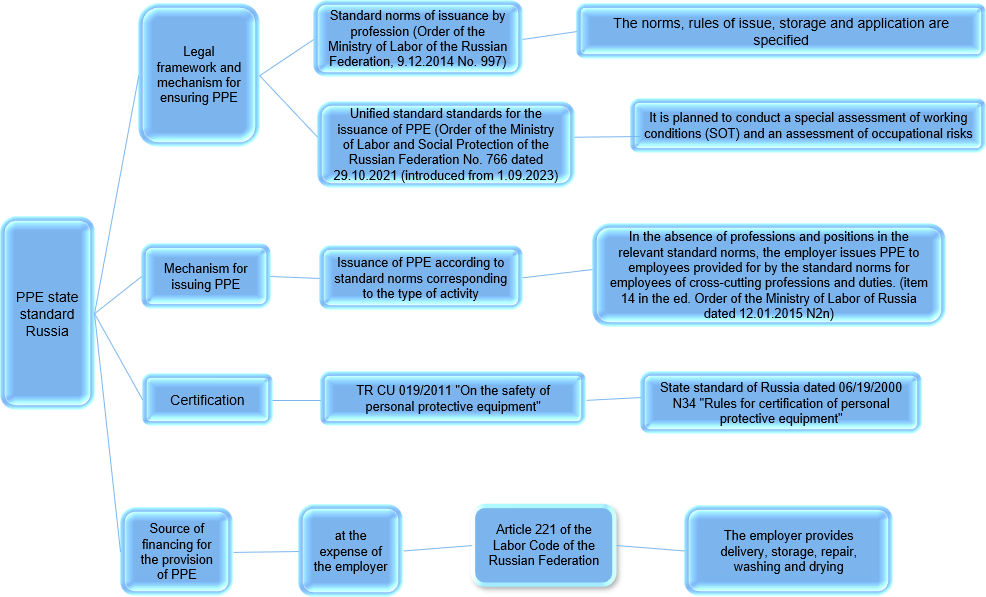
\includegraphics[width=0.8\textwidth]{media/chem2/image2}
	\caption*{Fig. 1 - Mechanism for Providing and Issuing PPE in Russia}
\end{figure}

\begin{figure}[H]
	\centering
	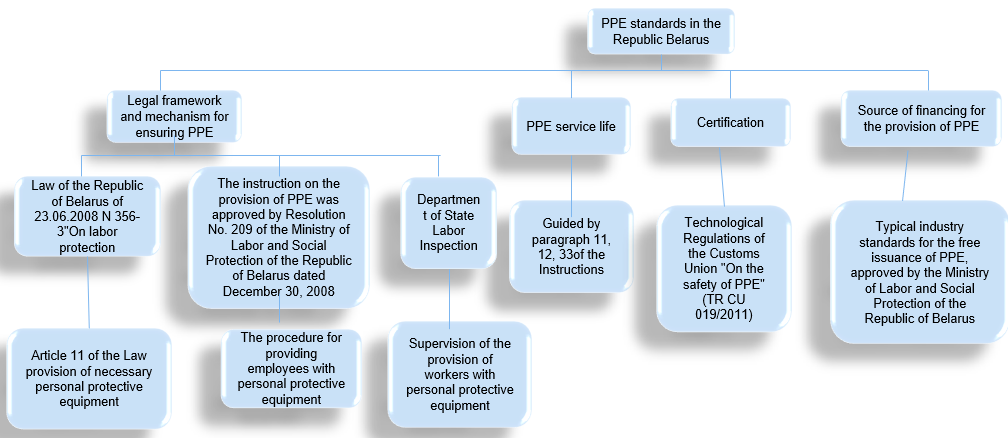
\includegraphics[width=0.8\textwidth]{media/chem2/image3}
	\caption*{Fig. 2 - Mechanism for Providing and Issuing PPE in the Republic of Belarus}
\end{figure}

\begin{multicols}{2}
{\bfseries Materials and methods.} The theoretical and methodological basis
of the study was based on regulatory documents, scientific works and
developments of domestic and foreign scientists on the use of PPE
against the impact of harmful and hazardous production factors and their
selection based on RBA {[}8{]}.

The results of the review revealed that in the post-Soviet countries
(RF, RB, RK) PPE and its components must comply with the requirements of
the Technical Regulations of the Customs Union "On the safety of
personal protective equipment" (hereinafter - TR CU019/2011) {[}9{]}.

In the Russian Federation, there are currently standard standards for
the issuance of PPE for 195 professions in accordance with the Order of
the Ministry of Labor of Russia dated December 9, 2014 "On approval of
standard standards for the free issuance of special clothing, special
footwear and other personal protective equipment to workers of
cross-cutting professions and positions of all types of economic
activity engaged in work with harmful and (or) hazardous working
conditions, as well as in work performed in special temperature
conditions or associated with pollution" {[}10{]}, which specifies the
standards, rules for the issuance, storage and use of PPE. In the
Republic of Belarus, the procedure for providing workers with PPE is
regulated by the Instructions for Providing Workers with PPE. Figures 1
and 2 show the mechanisms for providing and issuing PPE in Russia and
the Republic of Belarus, respectively.

Based on the results of the review of best practices in PPE provision
mechanisms using the example of Canada, the USA, Great Britain, Poland,
and Japan {[}11-17{]}, two countries from the North American continent
were identified as leaders.

The priority in ensuring occupational safety in Canada is the
organization of preventive measures, i.e., the reduction and elimination
of hazards. PPE is designed to protect against safety and/or health
threats. For example, helmets, safety glasses, and safety boots are
designed to prevent or reduce the severity of injury in case of
emergency (Figure 3).
\end{multicols}

\begin{figure}[H]
	\centering
	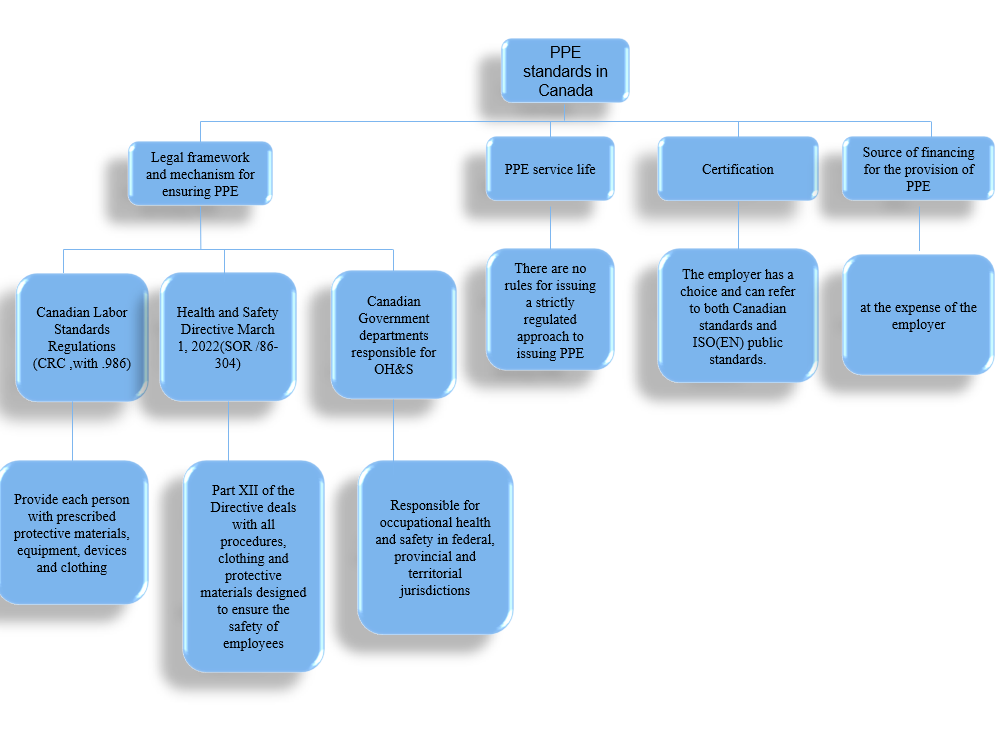
\includegraphics[width=0.7\textwidth]{media/chem2/image4}
	\caption*{Fig. 3 - Mechanism for providing and issuing PPE in Canada}
\end{figure}

\begin{multicols}{2}
The type and nature of hazards in the workplace in the USA are the main
indicators of the correct choice of PPE purchased at the
employer' s expense {[}12{]}. At the same time, employees
are given instructions on the risks that can be avoided or limited by
using PPE, the reasons for using PPE, how to use it safely and
effectively, and the actions to maintain it in good condition, such as
cleaning, replacing, storing (Figure 4).

In the UK, eliminating the hazard is the most effective way to manage
risks. According to the PPE provision policy (Figure 5), after
conducting a risk assessment using various control levels, the employer
is obliged to provide PPE to its employees at its own expense {[}13{]}.
\end{multicols}

\begin{figure}[H]
	\centering
	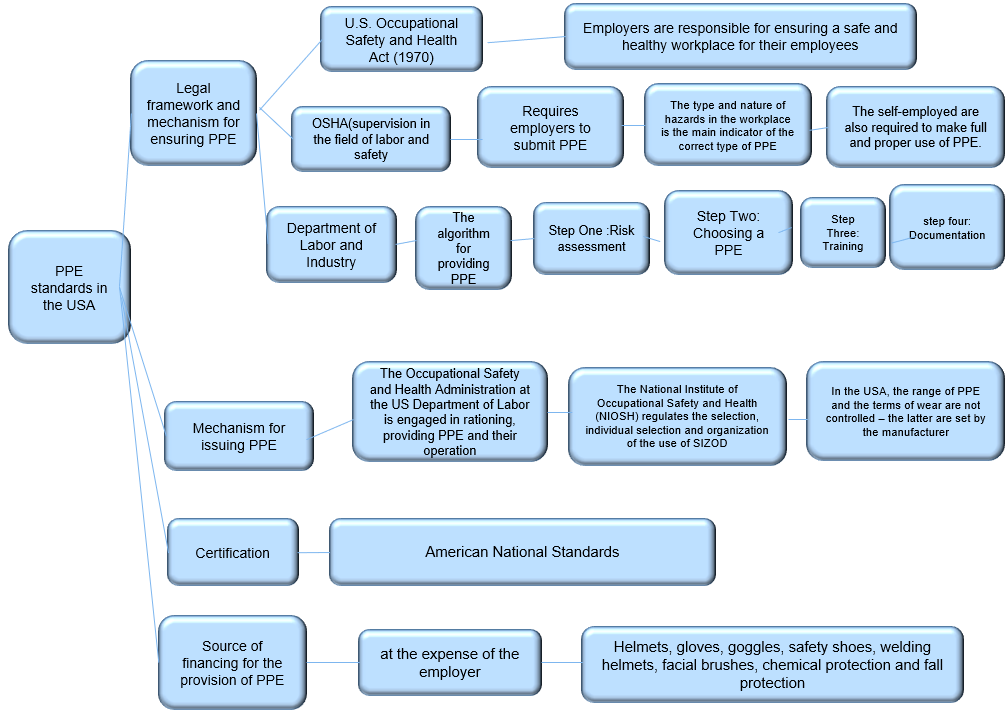
\includegraphics[width=0.85\textwidth]{media/chem2/image5}
	\caption*{Fig. 4 - PPE provision and issue mechanism in the USA}
\end{figure}

\begin{figure}[H]
	\centering
	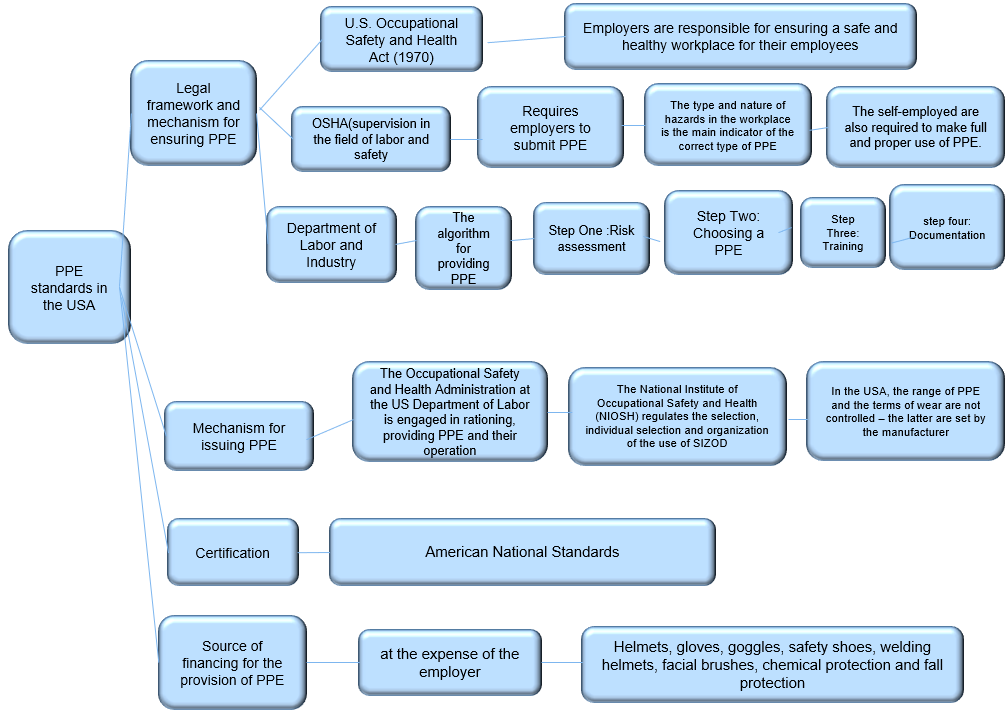
\includegraphics[width=0.85\textwidth]{media/chem2/image5}
	\caption*{Fig. 5 - PPE provision and issue mechanism in the UK}
\end{figure}

\begin{multicols}{2}
In the EU countries, the conformity assessment processes for personal
protective equipment are carried out only in accordance with the EU
Regulation 2016/425. Thus, in Poland they must also comply with the
requirements specified in the Act dated August 30, 2002 "On the
Conformity Assessment System" {[}14{]}. In Japan, the regulations on the
provision of PPE are based on risk assessment (Figure 6). According to
the requirements of the Occupational Safety and Health Act, Japanese
employers are required to independently develop accident prevention
programs at work and determine what protective equipment they will use
to prevent accidents {[}16{]}.
\end{multicols}

\begin{figure}[H]
	\centering
	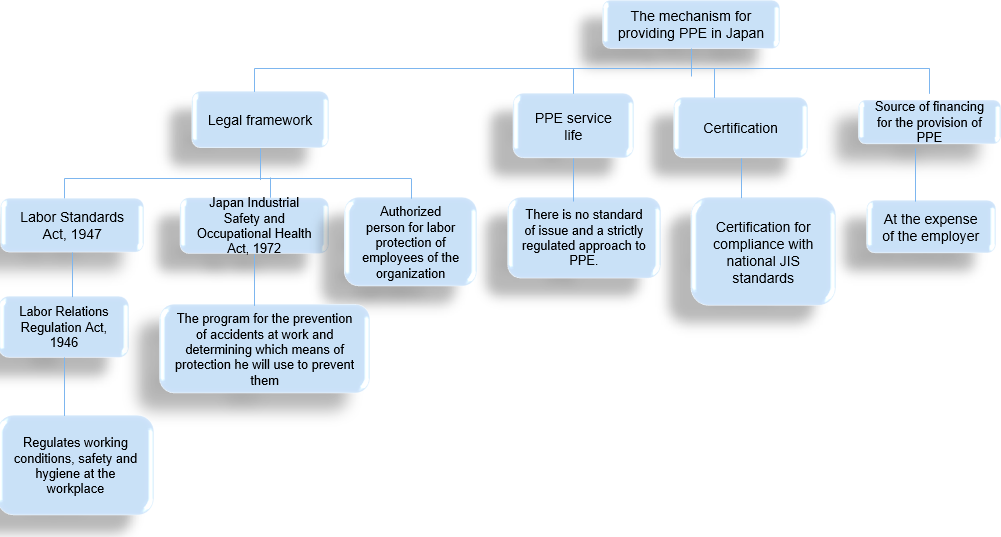
\includegraphics[width=0.85\textwidth]{media/chem2/image6}
	\caption*{Fig. 6 - Mechanism for providing and issuing PPE in Japan}
\end{figure}

\begin{figure}[H]
	\centering
	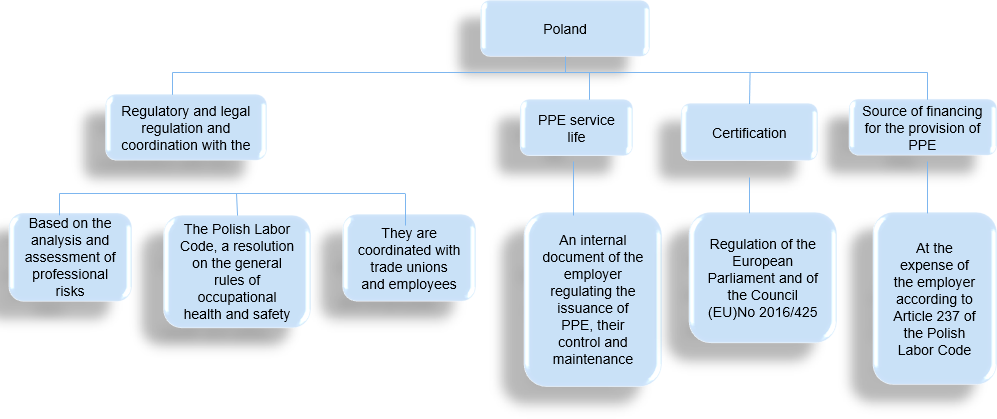
\includegraphics[width=0.85\textwidth]{media/chem2/image7}
	\caption*{Fig. 7 - Mechanism for providing and issuing PPE in Poland}
\end{figure}

\begin{multicols}{2}
Mixed/hybrid approach -- is currently typical for providing PPE in
Poland (Figure 7) and Russia. In Poland {[}14{]}, according to the Labor
Code, the employer determines the types of personal protective
equipment, as well as work clothes and footwear, the use of which is
required in certain positions. At the same time, this is done on the
basis of the Resolution of the Minister of Labor and Social Policy of
September 26, 1997 "On General Rules for Occupational Health and
Safety", which contains detailed rules for the use of PPE, including a
list of risks that require personal protective equipment (``Types of
work requiring the use of personal protective equipment with an
indication and decoding of the types of personal protective
equipment''). At the same time, the period of wear and operation is
determined based on the manufacturer' s requirements
provided in the documentation for the PPE. Accordingly, the regulatory
framework for the list of risks imposes on the employer an obligation to
assess the professional risk of each employee, which is provided for by
the Labor Code.

Thus, the employer of any enterprise must develop and approve by a local
act the standards for the free issuance of PPE to employees, based on
the Unified Standard Standards, taking into account the results of the
special assessment of working conditions, the results of the assessment
of professional risks, the opinion of the representative body of
employees. These standards can be developed by the enterprise itself, as
well as by involving third-party organizations or specialists {[}14{]}.

Based on the results of the analysis, the mechanisms and features of the
legal regulation of the provision of PPE were grouped as follows:

The list approach, which is based on strict regulatory consolidation of
the list of professions and types of work, for which PPE is provided,
sets and wearing periods are regulated, in some cases, provision in
excess of standards is prohibited. Regulation is carried out on an
industry basis, equalizing the working conditions of employees without
taking into account the actual state and measures taken by the employer
to improve working conditions (change in technology, technical
re-equipment, use of collective protective equipment, exclusion of
employee employment directly in the zone of exposure to harmful factors,
etc.). Approval of standards by an act of the employer is formal in
nature, the assessment of the provision of PPE consists in comparing it
with uniform/industry standards. This approach is observed in
post-Soviet countries such as Russia, Belarus, Kazakhstan.

Risk-oriented approach, which is based on mandatory assessment of the
professional risk of a specific employee. The provision of PPE is not
standardized at the legislative level, but the
employer' s responsibilities to ensure the protection of
employees are legislatively established. However, there are certain PPE
that are presented in the standards for specific works (helmet and
high-visibility vest for loading and unloading works without the
obligation to provide special clothing against contamination, etc.)
{[}18-21{]}. The standards for issuing and the terms of
wearing/operation of PPE are tied to the information contained in the
technical documentation for a specific product. The role of employee
representatives in this aspect is very important, since the formation of
the PPE register by the employer is carried out with their
participation/agreement, often with the agreement of the employee
himself. This approach is used in Canada, the USA, Great Britain, and
Japan.

A mixed/hybrid approach, which is currently typical for providing PPE in
Poland and Russia. In Poland, according to the Labor Code, the employer
determines the types of personal protective equipment, as well as work
clothes and footwear, the use of which is required in certain positions.
At the same time, this is done on the basis of the Resolution of the
Minister of Labor and Social Policy of September 26, 1997 "On General
Rules for Occupational Health and Safety" {[}15{]}, which contains
detailed rules for the use of PPE, including a list of risks that
require personal protective equipment (``Types of work requiring the use
of personal protective equipment with an indication and decoding of the
types of personal protective equipment''). At the same time, the period
of wear and operation is determined based on the
manufacturer' s requirements, given in the documentation
for the PPE. Accordingly, the regulatory framework for the list of risks
imposes on the employer an obligation to assess the professional risk of
each employee, which is provided for by the Labor Code.

Russia is in a transitional stage from the list approach and the hybrid
approach used alongside it, characterized by legislative regulation of
the procedure for providing PPE (Rules, Standard Standards) without
taking into account the industry focus. The key reform provides for the
transition from Standard Industry Standards for the Issuance of PPE
(more than 60 documents) in favor of Uniform Standard Standards
acceptable for all industries and sectors of the economy, which indicate
the names of professions, names and types of PPE, their quantities per
year. Risk-focused approach consists in introducing standards for the
issuance of PPE depending on the hazards that pose a threat to the life
and health of workers. A separate appendix provides the names of hazards
identified based on the results of the assessment of professional risks,
PPE that must be issued with a possible design, additional elements and
quantity per year. The approved standards serve as the basis for local
regulations at enterprises.

{\bfseries Results and discussion.} At the same time, the
employer' s obligation to use certified PPE remains a
single regulated requirement for all approaches. There is a significant
regulatory and technical framework, standards, bodies for confirming
product compliance with safety and quality requirements, and state
control is carried out.

The study found that to ensure occupational safety, it is necessary to
identify hazards, subsequently assess the risk of their impact, and
provide protective equipment taking into account the risk. The basis for
identifying hazards is the classification of hazardous and harmful
production factors. It is necessary to highlight those features that
will allow the best identification of hazardous and harmful production
factors, assess the risks of their impact on the
worker' s body, develop protective measures and implement
them in practice, thereby preventing injuries and diseases associated
with the employee' s work and the
employer' s production activities. Based on the
classification, it is possible to fully and reliably identify hazards in
the workplace {[}21-24{]}.

In this regard, in the course of scientific work, a classifier of risks
associated with the impact of production factors on the
worker' s body was developed (Table 1-2) {[}25,26{]}.
\end{multicols}

\begin{longtblr}[
  caption = {\bfseries Table 1 - Classifier of harmful and hazardous production factors},
  label = none,
  entry = none,
]{
  colspec = {X[0.3] X[0.5] X[5] X[0.6]},
  column{even} = {c},
  column{1} = {c},
  hlines,
  vlines,
}
{\textbf{}\\\textbf{No.}} & {\textbf{Factor}\\\textbf{code}} & \textbf{Name of risks associated with factors of the production environment}                          & {\textbf{Need to}\\\textbf{provide}\\\textbf{PPE (+/-)}} \\
1                         & \textbf{1}                       & \textbf{Impact of industrial factors of mechanical nature}                                            &                                                          \\
2                         & \textbf{1.1}                     & \textbf{Fall in the work area}                                                                        &                                                          \\
3                         & 1.1.1                            & Fall from a height or to a depth                                                                      & +                                                        \\
4                         & 1.1.2                            & Fall when slipping on slippery surfaces                                                               & +                                                        \\
5                         & 1.1.3                            & Fall, collapse, avalanche of objects (solid, liquid or gaseous objects)                               & +                                                        \\
6                         & 1.1.4                            & Fall, destruction of buildings, structures and their elements                                         & +                                                        \\
7                         & \textbf{1.2}                     & \textbf{Road accident}                                                                                &                                                          \\
8                         & 1.2.1                            & Vehicle collision                                                                                     & +                                                        \\
9                         & 1.2.2                            & Transport accidents                                                                                   & -                                                        \\
10                        & \textbf{1.3}                     & \textbf{Impact of production equipment}                                                               &                                                          \\
11                        & 1.3.1                            & Moving and rotating parts of equipment, mechanisms, machines, tools (impacts, grips, crushing)        & +                                                        \\
12                        & 1.3.2                            & Stationary cutting parts of production equipment, mechanisms, machines, tools (cuts, scratches)       & +                                                        \\
13                        & 1.3.3                            & Impact of high surface temperatures of equipment, mechanisms, machines, tools, liquids, gases, vapors & +                                                        \\
14                        & 1.3.4                            & Impact of low surface temperatures of equipment, mechanisms, machines, tools                          & +                                                        \\
15                        & \textbf{2}                       & \textbf{Impact of production factors of a physical nature}                                            &                                                          \\
16                        & \textbf{2.1}                     & \textbf{Impact of electric current}                                                                   &                                                          \\
17                        & 2.1.1                            & Electric shock from equipment, mechanisms, machines, tools                                            & +                                                        \\
18                        & 2.1.2                            & Impact of an electric arc                                                                             & +                                                        \\
19                        & \textbf{2.2}                     & \textbf{Risk of fire or explosion}                                                                    &                                                          \\
20                        & 2.2.1                            & Ignition of flammable substances                                                                      & +                                                        \\
21                        & 2.2.2                            & Static electricity                                                                                    & +                                                        \\
22                        & 2.2.3                            & Exposure to smoke, steam, harmful gases and dust                                                      & +                                                        \\
23                        & 2.2.4                            & Working with pressure vessels                                                                         & +                                                        \\
24                        & \textbf{2.3}                     & \textit{\textbf{Climate/microclimate}}                                                                &                                                          \\
25                        & 2.3.1                            & Increased air temperature in open areas                                                               & +                                                        \\
26                        & 2.3.2                            & Decreased air temperature in open areas                                                               & +                                                        \\
27                        & 2.3.3                            & Increased air velocity in open areas                                                                  & +                                                        \\
28                        & 2.3.4                            & Increased air humidity in open areas                                                                  & +                                                        \\
29                        & 2.3.4                            & Increased air temperature indoors                                                                     & +                                                        \\
30                        & 2.3.4                            & Decreased air temperature indoors                                                                     & +                                                        \\
31                        & 2.3.4                            & Increased air velocity indoors                                                                        & +                                                        \\
32                        & 2.3.4                            & Increased air humidity indoors                                                                        & +                                                        \\
33                        & 2.3.4                            & Increased thermal radiation                                                                           & +                                                        \\
34                        & 2.3.4                            & Increased atmospheric pressure                                                                        & -                                                        \\
35                        & \textbf{2.4}                     & \textit{\textbf{Ionizing radiation}}                                                                  &                                                          \\
36                        & 2.4.1                            & Alpha radiation                                                                                       & \textit{\textbf{+}}                                      \\
37                        & 2.4.2                            & Beta radiation                                                                                        & \textit{\textbf{+}}                                      \\
38                        & 2.4.3                            & Gamma radiation (expository)                                                                          & \textit{\textbf{+}}                                      \\
39                        & 2.4.4                            & X-ray radiation                                                                                       & \textit{\textbf{+}}                                      \\
40                        & 2.4.5                            & Electrically charged air particles - aeroions                                                         & \textit{\textbf{+}}                                      
\end{longtblr}

The proposed classifier consists of 6 main groups, 19 names, and 55
subgroups of production factors, and its application is substantiated
using examples.

\begin{longtblr}[
  caption = {\bfseries Table 2 - Classifier of harmful and hazardous production factors},
  label = none,
  entry = none,
]{
  colspec = {X[0.3] X[0.5] X[5] X[0.6]},
  column{even} = {c},
  column{1} = {c},
  hlines,
  vlines,
}
\textbf{No.} & {\textbf{Factor}\\\textbf{code}} & \textbf{Name of risks associated with factors of the production environment}                                                         & {\textbf{Need to}\\\textbf{provide}\\\textbf{PPE (+/-)}} \\
 1             & \textbf{2.5}                     & \textit{\textbf{Non-ionizing radiation}}                                                                                             &                                                          \\
 2             & 2.5.1                            & Electrostatic field                                                                                                                  & +                                                        \\
 3             & 2.5.2                            & Permanent magnetic field (including hypogeomagnetic)                                                                                 & +                                                        \\
 4             & 2.5.3                            & Industrial frequency electric and magnetic fields                                                                                    & +                                                        \\
 5             & 2.5.4                            & Broadband electromagnetic fields generated by personal computers                                                                     & -                                                        \\
 6             & 2.5.5                            & Infrared radiation                                                                                                                   & \textbf{+}                                               \\
 7             & 2.5.6                            & Ultraviolet radiation                                                                                                                & +                                                        \\
 8             & 2.5.7                            & Laser radiation                                                                                                                      & +                                                        \\
 9             & \textbf{2.6}                     & \textit{\textbf{Vibroacoustic factors}}                                                                                              &                                                          \\
 10            & 2.6.1                            & Continuous noise                                                                                                                     & +                                                        \\
 11            & 2.6.2                            & Pulsed noise                                                                                                                         & +                                                        \\
 12            & 2.6.3                            & General vibration                                                                                                                    & +                                                        \\
 13            & 2.6.4                            & Local vibration                                                                                                                      & +                                                        \\
 14            & 2.6.5                            & Infrasound                                                                                                                           & +                                                        \\
 15            & 2.6.6                            & Ultrasound                                                                                                                           & +                                                        \\
 16            & \textbf{2.7}                     & \textit{\textbf{Light environment}}                                                                                                  &                                                          \\
 17            & 2.7.1                            & Insufficient illumination of the work area                                                                                           & +                                                        \\
 18            & 2.7.2                            & Increased illumination of the work area (brightness of light, direct and reflected, increased pulsation of the light flux)           & +                                                        \\
 19            & \textbf{2.8}                     & \textit{\textbf{Aerosol composition of air}}                                                                                         &                                                          \\
 20            & 2.8.1                            & Highly and moderately fibrogenic aerosols                                                                                            & +                                                        \\
 21            & 2.8.2                            & Low-fibrogenic aerosols                                                                                                              & +                                                        \\
 22            & \textbf{3}                       & \textbf{Impact of industrial factors of chemical nature}                                                                             &                                                          \\
 23            & 3.1                              & \textit{\textbf{Chemical substances contained in the air of the working area (aerosols, vapors, gases, fumes)}}                      &                                                          \\
 24            & 3.1.1                            & Acute toxicity substances                                                                                                            & \textbf{+}                                               \\
 25            & 3.1.2                            & Irritant substances                                                                                                                  & \textbf{+}                                               \\
 26            & 3.1.3                            & Carcinogenic substances                                                                                                              & \textbf{+}                                               \\
 27            & 3.1.4                            & Allergenic substances                                                                                                                & \textbf{+}                                               \\
 28            & 3.1.5                            & Substances hazardous to reproductive health                                                                                          & \textbf{+}                                               \\
 29            & 3.1.6                            & Substances prohibited for inhalation and skin contact (antitumor drugs, estrogen hormones, narcotic analgesics)                      & \textbf{+}                                               \\
 30            & 3.1.7                            & Solutions of acids, alkalis, etc., solid and bulk substances that affect the skin and mucous membranes                               & \textbf{+}                                               \\
 31            & \textbf{4}                       & \textbf{Impact of production factors of biological nature}                                                                           &                                                          \\
 32            & 4.1                              & Microorganisms-producers, preparations containing living cells and spores of microorganisms                                          & +                                                        \\
 33            & 4.2                              & Pathogenic microorganisms and viruses (causative agents of especially dangerous and other infectious diseases)                       & +                                                        \\
 34            & 4.3                              & Getting of poisons, waste products and plants themselves, insects, arachnids, animals on the skin and inside the body                & +                                                        \\
 35            & \textbf{5}                       & \textbf{Impact of production factors of psychophysiological nature}                                                                  &                                                          \\
 36            & 5.1                              & Difficulty of labor                                                                                                                  & -                                                        \\
 37            & 5.2                              & Intensity of labor                                                                                                                   & -                                                        \\
 38            & \textbf{6}                       & \textbf{Exposure to general industrial contaminants}                                                                                 &                                                          \\
 39            & 6.1                              & Water (including contaminated) and solutions of non-toxic substances (dyes, adhesives, oily and other substances) and labor products & +                                                        \\
 40            & 6.2                              & Non-toxic dust (fine chips, small fragments, coarse dust)                                                                            & +                                                        
\end{longtblr}

\begin{multicols}{2}
The classifier contains the following main names of risks associated
with the impact of factors of the production environment and the work
process on the worker' s body:

- impact of production factors of a mechanical nature (fall in the work
area, road traffic accident, impact of production equipment);

- impact of production factors of a physical nature (electric current,
threat of fire or explosion, climate/microclimate, ionizing radiation,
non-ionizing radiation, vibroacoustic factors, light environment,
aerosol composition of air);

- impact of production factors of a chemical nature (chemical substances
contained in the air of the working area (aerosols, vapors, gases,
fumes);

- impact of production factors of a biological nature (microorganisms -
producers, pathogenic microorganisms and viruses, waste products of
plants, insects, arachnids, animals);

- impact of production factors of a psychophysiological nature (severity
of work, labor intensity);

- impact of general industrial pollutants (water and solutions of
non-toxic substances, non-toxic dust)

{\bfseries Conclusions.} Analysis of the current mechanisms for providing
PPE in the Republic of Kazakhstan has established that regulation is
determined by 22 industries and 3,544 professions based on approved
standards for issuing special clothing and other personal protective
equipment to employees of organizations of various types of economic
activity.

Compliance with the established standards in practice puts the employer
in a strict framework, on the one hand, with the need to purchase PPE
that is inadequate for working conditions, on the other hand, with the
impossibility of increasing/decreasing the wearing period and quantity,
changing the completeness, etc. The domestic mechanism for providing PPE
is characterized by a ``list'' approach and strict regulation of the
types of PPE depending on the profession or position of the employee,
which in some cases leads to the creation of barriers in ensuring safe
work at enterprises. At the same time, the experience of developed
countries shows the effectiveness of using RBA in providing PPE.

Thus, developed foreign countries use models for providing PPE based on
an assessment of professional risks, analyzing specific hazards and
providing relevant means of protection against them. The introduction of
risk assessment into the labor legislation of the Republic of Kazakhstan
and the existing regulatory mechanism for the provision of PPE, which
does not take into account the specifics of the labor process and the
presence/absence of harmful production factors and professional risks,
requires revision. It is assumed that based on the results of the
assessment of professional risks, as well as taking into account the
physical, chemical, biological factors of the production environment and
factors of the labor process, employers should be able to independently
develop and approve standards for providing PPE to employees of the
enterprise {[}2{]}.

In this regard, it is necessary to improve the current regulatory
mechanism for providing special clothing, footwear and other PPE with
increased flexibility in determining the contingent of employees,
choosing protective equipment, assigning additional sets, replacement
and complex PPE, service life.

Thus, the employer of any enterprise must develop and approve by a local
act the standards for the free issuance of PPE to employees, based on
the unified standard guidelines, taking into account the results of the
special assessment of working conditions, the results of the assessment
of professional risks, the opinion of the representative body of
employees. These standards can be developed by the enterprise itself, or
by involving third-party organizations or specialists.

Considering that the range of modern PPE fully covers protection against
all possible factors of the production environment and professional
risks, a methodology for providing PPE based on RBA will be developed
and implemented, as well as a nomenclature of PPE corresponding to the
degree and type of exposure to harmful and (or) hazardous production
factors {[}2{]}.

Also, based on the results of the study, a classifier of risks
associated with the impact of production factors on the
worker' s body, as well as a classifier of harmful and
hazardous production factors were developed.

\emph{{\bfseries Financing:}} \emph{This research has been/was/is funded by
the Science Committee of the Ministry of Education and Science of the
Republic of Kazakhstan (Grant No. BR22182667 ``Working Conditions and
Occupational Risks: Classification, Categories, and Grouping Criteria in
the Transition to the "Green Economy").}
\end{multicols}

\begin{center}
{\bfseries References}
\end{center}

\begin{references}
1. Labor Code of the Republic of Kazakhstan. Code of the Republic of
Kazakhstan dated November 23, 2015 No. 414-V ZRK.
\href{https://adilet.zan.kz/rus/docs/K1500000414}{https://adilet.zan.kz}.Data obrashhenija:
13.10.2024. {[}in Russian{]}.

2. Risk-orientirovannyj podhod k obespecheniju sredstvami
individual' noj zashhity na predprijatii // Kollektiv
avtorov pod redakciej Abikenovoj Sh.K. Nauchno-informacionnoe izdanie.
ISBN 978-601-08-2792-9. -- Nur-Sultan: RGP na PHV ``RNIIOT MTSZN RK'',
2022. -220 s.{[}in Kazakh{]}.

3. Personal Protective Equipment and the Role of a Trained Observer,
NETEC {[}URL:\\
\href{http://file.lacounty.gov/SDSInter/dhs/1068461_SlideDeck5-PPEandInfectionControlPrinciples.pdf}{http://file.lacounty.gov}{]}.
Data obrashhenija:13.10.2024.

4. Foster, J., Hodder, S.G., Goodwin, J., Havenith, G. (2020).
Occupational heat stress and practical cooling solutions for healthcare
and industry workers during the COVID-19 pandemic// Ann Work Expo
Health.- 2022.-Vol.64(9).- P. 915-922. DOI 10.1093/annweh/wxaa082

5. Zakon Respubliki Kazahstan ``O biologicheskoj bezopasnosti Respubliki
Kazahstan'' Postanovlenie \\Pravitel' stva Respubliki
Kazahstan ot 21 maja 2022 goda № 122-VII ZRK
\href{https://adilet.zan.kz/rus/docs/Z2200000122}{https://adilet.zan.kz}. {[}in Russian{]}. (Data
obrashhenija: 28.04.2022).

6. Ortega, R., Gonzalez, M., Nozari, A., \& Canelli, R. (2020). Personal
Protective Equipment and Covid-19//The New England journal of
medicine.-2020.- Vol. 382(26).- e105. DOI 10.1056/NEJMvcm2014809

7. Pritchard, A. (2020). Personal protective equipment//Australian
journal of general practice/-2020. DOI 10.31128/AJGP-COVID-07

8. Tehnicheskie reglamenty Tamozhennogo sojuza. O bezopasnosti sredstv
individual' noj zashhity (TR TS 019/2011) / Prinjat
resheniem Komissii Tamozhennogo sojuza ot 9 dekabrja 2011 g. № 878.\\
\href{https://adilet.zan.kz/rus/docs/H11T0000878}{https://adilet.zan.kz}. {[}in Russian{]}. Data
obrashhenija: 30.10.2024.

9.Prikaz Ministerstva truda i social' noj zashhity
Rossijskoj Federacii ot 9 dekabrja 2014 g. «Ob \\utverzhdenii tipovyh norm
besplatnoj vydachi special' noj odezhdy,
special' noj obuvi i drugih sredstv
individual' noj zashhity rabotnikam skvoznyh professij i
dolzhnostej vseh vidov jekonomicheskoj dejatel' nosti,
zanjatym na rabotah s vrednymi i (ili) opasnymi uslovijami truda, a
takzhe na rabotah, vypolnjaemyh v osobyh temperaturnyh uslovijah ili
svjazannyh s zagrjazneniem»
\href{https://normativ.kontur.ru/document?moduleId=1\&documentId=247205}{https://normativ.kontur.ru}. {[}in
Russian{]}. Data obrashhenija: 30.10.2024.

10. Prikaz Ministerstva truda i social' noj zashhity
Rossijskoj Federacii ot 16.11.2020 № 782n. "Ob utverzhdenii Pravil po
ohrane truda pri vypolnenii rabot na vysote"
\href{https://normativ.kontur.ru/document?moduleId=1\&documentId=379253\&ysclid=l9u855zqyi192989478}{https://normativ.kontur.ru}.
{[}in Russian{]}. Data obrashhenija: 30.10.2024.

11. Technical Report TR-0200 (4230-46)-3. Aerospace Corporation, Los
Angeles, California, USA. The Infrastructure Health and Safety
Association (IHSA) \href{https://www.ihsa.ca/topics_hazards/ppe.aspx}{https://www.ihsa.ca}.
Date of access: 30.10.2024.

12. Occupational Safety and Health Administration: Employer Payment for
Personal Protective Equipment; Final Rule.
\href{https://www.osha.gov/laws-regs/federalregister/2007-11-15-0}{https://www.osha.gov}. Date
of access: 02.12.2024.

13. Rules for using PPE in the UK. UK Statutory Instruments, 2022 No. 8:
The Personal Protective Equipment at Work (Amendment) Regulations 2022.
\href{https://www.hse.gov.uk/ppe/ppe-regulations-2022.htm\#:\textasciitilde:text=Under\%20PPER\%202022\%2C\%20the\%20types,on\%20the\%20use\%20of\%20PPE}{https://www.hse.gov.uk}.
Date of access:11.01.2025.

14. Law of August 30, 2002 on the conformity assessment system.
{[}Electronic resource{]}.\\
\href{https://isap.sejm.gov.pl/isap.nsf/DocDetails.xsp?id=WDU20021661360}{https://isap.sejm.gov.pl}. Date
of access: 11.01.2025.

15. Decree of the Minister of Labor and Social Policy Poland Republic of
September 26, 1997. On general rules of labor protection and safety at
work.
\href{https://www.global-regulation.com/translation/poland/2986216/regulation-of-the-minister-of-labour-and-social-policy-of-26-september-1997-on-general-provisions-of-occupational-safety-and-health.html}{https://www.global-regulation.com}
Date of access: 30.10.2024.

16. Japan International Cooperation Agency. JICA standard safety
specification (JSSS).\\
\href{https://www.jica.go.jp/Resource/english/our\_work/types\_of\_assistance/c8h0vm00008zx0m8-att/jsss\_01.pdf}{https://www.jica.go.jp}.
Date of access: 08.01.2025

17. Vukicevic, A.M., Djapan, M., Isailovic, V., Milasinovic, D.,
Savkovic, M., Milosevic, P. (2022). Generic compliance of industrial PPE
by using deep learning techniques// Safety Sci.-
2020.-Vol.148(5) : 105646. DOI 10.1016/j.ssci.2021.105646

18. Balamurugan, B., Grant, R., Gaurav N. PPE Compliance Detection using
Artificial Intelligence in Learning Factories //Procedia
Manufacturing.-2020.- Vol.45.- P.277-282. DOI\\
10.1016/j.promfg.2020.04.017

19. Kursunoglu, N., Onder, S., Onder, M. (2022). The Evaluation of
Personal Protective Equipment Usage Habit of Mining Employees Using
Structural Equation Modeling//Safety and Health at
Work.-2022.-Vol.13(2).- P. 180-186. DOI 10.1016/j.shaw.2022.03.004

20. Jack C.P.Cheng, Peter Kok-YiuWong, Han Luo et al. Vision-based
monitoring of site safety compliance based on worker re-identification
and personal protective equipment classification//Automation in\\
Construction.-2022.-Vol.139. DOI 10.1016/j.autcon.2022.104312

21. Sholpan Abikenova, Gulnara Issamadiyeva, Elmira Kulmagambetova,
Gulzhan Daumova, Nazgul \\Abdrakhmanova. Assessing Occupational Risk: A
Classification of Harmful Factors in the Production Environment and
Labor Process // International Journal of Safety and Security
Engineering. -2023ю Vol. 13(5).- P.871-881 DOI10.18280/ijsse.130511\\
22. GOST 12.0.003-2015 ``Systema standartov po ohrane truda. Opasnye I
vrednye proizvodstvennye factory. Klassifikacya" GOST RK
\href{https://online.zakon.kz/Document/?doc_id=34182412}{https://online.zakon.kz} {[}in
Russian{]}. Data obrashhenija: 11.01.2025)

23. Opasnye i vrednye proizvodstvennye faktory. {[}Jelektronnyj
resurs{]}.
\href{https://nalog-nalog.ru/ohrana_truda/opasnye_i_vrednye_proizvodstvennye_faktory_perechen}{https://nalog-nalog.ru}{]}.
{[}in Russian{]}. Data obrashhenija: 15.10.2024

24. Metodicheskie rekomendacii: Gigienicheskie kriterii ocenki i
klassifikacija uslovij truda po \\pokazateljam vrednosti i opasnosti
faktorov proizvodstvennoj sredy, tjazhesti i intensivnosti trudovogo
processa. Utverzhdeno prikazom Predsedatelja Komiteta
sanitarno-jepidemiologicheskogo nadzora \\Ministerstva zdravoohranenija
Respubliki Kazahstan ot 31 dekabrja 2020 goda № 24.\\
\href{https://online.zakon.kz/Document/?doc\_id=35193093}{https://online.zakon.kz}{]}. {[}in Russian{]}.
Data obrashhenija: 15.10.2024.

25. A.S. № 28600 ot 06.09.2022 g. Nomenklatura sredstv
individual' noj zashhity v zavisimosti ot vrednyh
proizvodstvennyh faktorov i stepeni ih vozdejstvija /
Zajavitel': Respublikanskij
nauchno-issledovatel' skij institut ohrany truda
Ministerstva truda i social' noj zashhity naselenija
Respubliki Kazahstan, Astana, 2022 g.

26.Abikenova Sh., Issmadiyeva G., Kulmagambetova E., Daumova G.
Assessing Occupational Risk: A Classification of Harmful Factors in the
Production Environment and Labor Process// International Journal of
Safety and Security Engineering.- 2023.-Vol/13(5).-P.871-881
DOI. 10.18280/ijsse.130511
\end{references}

\begin{authorinfo}
\emph{{\bfseries Information about the author}}

Bekmagambetov A.- higher law degree, candidate of legal sciences,
Associate Professor, REM with RSE Republican Research Institute for
Labor Protection of the Ministry of Labor and Social Protection of
Population of the Republic of Kazakhstan, Astana,Kazakhstan,e-mail:
Adilet1979@mail.ru;

Kulmagambetova E. - candidate of chemical science, Leading Researcher of
the Department of Monitoring and Occupational Health, REM with RSE
Republican Research Institute for Labor Protection of the Ministry of
Labor and Social Protection of Population of the Republic of Kazakhstan,
Astana, 010000, Republic of Kazakhstan,e-mail:
elya\_\href{mailto:kulmagambet@.mail.ruedu.kz}{kulmagambet@.mail.ru};

Madeniyet Y. - Candidate of Chemical Science, Dean of the Faculty of
Natural Sciences, Professor «Toraighyrov University» NCJSC, Pavlodar,
Kazakhstan, e-mail:
\href{mailto:yelubay.m@tou.edu.kz}{\nolinkurl{yelubay.m@tou.edu.kz}};

Rakhmetova A. - candidate of medical science, Associate Professor Head
of the Department of Monitoring and Occupational Health, REM with RSE
Republican Research Institute for Labor Protection of the Ministry of
Labor and Social Protection of Population of the Republic of Kazakhstan,
Astana, Kazakhstan,
e-mail:elya\_\href{mailto:ra_anar@.mail.ru}{\nolinkurl{ra\_anar@.mail.ru}};

Tolegenov D.- Researcher at the Department of Chemistry and Chemical
Technologies «Toraighyrov University»

NCJSC, Faculty of Natural Sciences, Pavlodar, Kazakhstan, e-mail:
\href{http://www.dika-92@mail.ru}{www.dika-92@mail.ru}

\emph{{\bfseries Сведения об авторах}}

Бекмагамбетов А.- кандидат юридических наук, ассоцированный профессор,
Республиканский научно -\\исследовательский институт по охране труда
Министерства труда и социальной защиты населения Республики Казахстан и.
о. генерального директора, e-mail: Adilet1979@mail.ru;

Кульмагамбетова Э.- кандидат химических наук, Республиканский
научно-исследовательский институт по охране труда Министерства труда и
социальной защиты населения Республики Казахстан, dедущий научный
сотрудник отдела биомониторинга и гигиены труда, e-mail:
elya\_\href{mailto:kulmagambet@.mail.ruedu.kz}{kulmagambet@.mail.ru};

Мадениет Е. - кандидат химических наук, профессор декан факультета
естественных наук, НАО «Торайгыров Университет»,Павлодар, Казахстан,
e-mail:
\href{mailto:yelubay.m@tou.edu.kz}{\nolinkurl{yelubay.m@tou.edu.kz}};

Рахметова A. - кандидат медицинских наук, доцент, Республиканский
научно-исследовательский институт по охране труда Министерства труда и
социальной защиты населения Республики Казахстан», руководитель отдела
биомониторинга и гигиены труда, Астана, Казахстан, e-mail:
elya\_\href{mailto:ra_anar@.mail.ru}{\nolinkurl{ra\_anar@.mail.ru}};

Төлегенов Д. {\bfseries -} научный сотрудник кафедры «Химия и химические
технологии», НАО «Торайгыров университет», факультет естественных наук,
Павлодар, Казахстан, e-mail:
\href{http://www.dika-92@mail.ru}{www.dika-92@mail.ru}
\end{authorinfo}
